\documentclass{beamer}

\usepackage[utf8]{inputenc}

\usetheme{Madrid}
\setbeamerfont{normal text}{size=\small}

\usecolortheme{default}
\usepackage{extarrows}
\usepackage{amsmath}
\usepackage{amssymb,amsfonts,amsthm}
\usepackage{txfonts}
\usepackage{tkz-euclide}
\usepackage{listings}
\usepackage{adjustbox}
\usepackage{array}
\usepackage{tabularx}
\usepackage{gvv}
\usepackage{lmodern}
\usepackage{circuitikz}
\usepackage{tikz}
\usepackage{graphicx}
\usepackage{multicol}
\usepackage{xcolor}

\setbeamertemplate{page number in head/foot}[totalframenumber]

% --- FIXED LISTINGS CONFIGURATION ---
\definecolor{backcolour}{gray}{0.95}
\definecolor{codegreen}{rgb}{0,0.6,0}
\definecolor{codegray}{rgb}{0.5,0.5,0.5}

\lstset{
    language=Python,
    backgroundcolor=\color{backcolour},
    basicstyle=\ttfamily\small,
    keywordstyle=\color{blue},
    stringstyle=\color{orange},
    commentstyle=\color{codegreen},
    numbers=left,
    numberstyle=\tiny\color{codegray},
    breaklines=true,
    showstringspaces=false,
    frame=single,
    rulecolor=\color{orange!70},
    keepspaces=true
}
% ------------------------------------

\title{Probability Mass Function and Expected Value}
\author{Kartik Lahoti : EE25BTECH11032}

\begin{document}

\begin{frame}
    \titlepage
\end{frame}

\begin{frame}
    \frametitle{Question}
    The random variable $X$ takes on the values 1, 2 or 3 with probabilities $\frac{2+5P}{5}$, $\frac{1+3P}{5}$, and $\frac{1.5+2P}{5}$, respectively. The values of $P$ and $E[X]$ are respectively:
    
    \vspace{0.5cm}
    \begin{multicols}{2}
        \begin{enumerate}[a)]
        \item $0.05, 1.87$
        \item $1.90, 5.87$
        \item $0.05, 1.10$
        \item $0.25, 1.40$
        \end{enumerate}
    \end{multicols}
\end{frame}

\begin{frame}
    \frametitle{Theory: Properties of a PMF}
    For any discrete random variable $X$, the Probability Mass Function (PMF) must satisfy two main properties:
    
    \vspace{0.3cm}
    \begin{enumerate}
        \item The probability of each outcome must be non-negative:
        \begin{align}
            P(X = x_i) \geq 0 \quad \text{for all } i
        \end{align}
        \item The sum of all probabilities over the entire sample space must equal 1:
        \begin{align}
            \sum_{i} P(X = x_i) = 1
        \end{align}
    \end{enumerate}
    
    \vspace{0.3cm}
    We will use the second property to find the unknown variable $P$.
\end{frame}

\begin{frame}
    \frametitle{Step 1: Finding the value of P}
    According to the sum of probabilities rule:
    \begin{align}
        P(X=1) + P(X=2) + P(X=3) &= 1
    \end{align}
    Substituting the given expressions:
    \begin{align}
        \frac{2+5P}{5} + \frac{1+3P}{5} + \frac{1.5+2P}{5} &= 1
    \end{align}
    Combine the numerators over the common denominator:
    \begin{align}
        \frac{(2 + 1 + 1.5) + (5P + 3P + 2P)}{5} &= 1 \\
        \frac{4.5 + 10P}{5} &= 1
    \end{align}
\end{frame}

\begin{frame}
    \frametitle{Step 1: Finding the value of P }
    Multiplying both sides by 5:
    \begin{align}
        4.5 + 10P &= 5
    \end{align}
    Subtracting 4.5 from both sides:
    \begin{align}
        10P &= 5 - 4.5 \\
        10P &= 0.5
    \end{align}
    Solving for $P$:
    \begin{align}
        P &= \frac{0.5}{10} = \mathbf{0.05}
    \end{align}
\end{frame}

\begin{frame}
    \frametitle{Step 2: Deriving the PMF}
    Now substitute $P = 0.05$ back into the original probability expressions to find the exact PMF:
    
    \vspace{0.3cm}
    For $X = 1$:
    \begin{align}
        P(X=1) &= \frac{2 + 5(0.05)}{5} = \frac{2 + 0.25}{5} = \frac{2.25}{5} = \mathbf{0.45}
    \end{align}
    
    For $X = 2$:
    \begin{align}
        P(X=2) &= \frac{1 + 3(0.05)}{5} = \frac{1 + 0.15}{5} = \frac{1.15}{5} = \mathbf{0.23}
    \end{align}
    
    For $X = 3$:
    \begin{align}
        P(X=3) &= \frac{1.5 + 2(0.05)}{5} = \frac{1.5 + 0.10}{5} = \frac{1.60}{5} = \mathbf{0.32}
    \end{align}
\end{frame}

\begin{frame}
    \frametitle{Step 3: Calculating Expected Value $E[X]$}
    The expected value of a discrete random variable is given by:
    \begin{align}
        E[X] = \sum_{x} x \cdot P(X=x)
    \end{align}
    
    Substitute the values from our derived PMF:
    \begin{align}
        E[X] &= (1 \cdot 0.45) + (2 \cdot 0.23) + (3 \cdot 0.32) \\
        E[X] &= 0.45 + 0.46 + 0.96 \\
        E[X] &= \mathbf{1.87}
    \end{align}
    
    \vspace{0.3cm}
    \textbf{Conclusion:}
    The values of $P$ and $E[X]$ are $0.05$ and $1.87$, respectively. This matches option \textbf{(a)}.
\end{frame}

\begin{frame}
    \frametitle{Step 4: Calculating the Cumulative Distribution Function (CDF)}
    The Cumulative Distribution Function, $F_X(x)$, represents the probability that the random variable $X$ will take a value less than or equal to $x$:
    \begin{align}
        F_X(x) = P(X \leq x) = \sum_{x_i \leq x} P(X = x_i)
    \end{align}
    
    Using our derived PMF, we accumulate the probabilities step-by-step:
    \vspace{0.2cm}
    \begin{itemize}
        \item \textbf{For $x < 1$:} $F_X(x) = 0$
        \item \textbf{For $1 \leq x < 2$:} $F_X(x) = P(X=1) = \mathbf{0.45}$
        \item \textbf{For $2 \leq x < 3$:} $F_X(x) = P(X=1) + P(X=2) = 0.45 + 0.23 = \mathbf{0.68}$
        \item \textbf{For $x \geq 3$:} $F_X(x) = 0.68 + P(X=3) = 0.68 + 0.32 = \mathbf{1.00}$
    \end{itemize}
\end{frame}

\begin{frame}
    \frametitle{Step 4: CDF Piecewise Function}
    Summarizing the calculations, we can formally write the CDF as a piecewise step function:
    
    \vspace{0.5cm}
    \begin{align}
        F_X(x) = 
        \begin{cases} 
            0, & \text{if } x < 1 \\ 
            0.45, & \text{if } 1 \leq x < 2 \\ 
            0.68, & \text{if } 2 \leq x < 3 \\ 
            1.00, & \text{if } x \geq 3 
        \end{cases}
    \end{align}
    
    \vspace{0.5cm}
    This perfectly matches the expected behavior of a CDF, where it starts at $0$ and monotonically increases to $1$.
\end{frame}

\begin{frame}[fragile]
    \frametitle{Python Code }
\begin{lstlisting}
import matplotlib.pyplot as plt
import numpy as np

X = np.array([1, 2, 3])
prob = np.array([0.45, 0.23, 0.32])

cdf = np.cumsum(prob)

fig, (ax1, ax2) = plt.subplots(1, 2, figsize=(14, 5))

ax1.stem(X, prob, basefmt=" ", linefmt='b-')
ax1.set_title('Probability Mass Function (PMF)', fontsize=14)
ax1.set_xlabel('Random Variable X', fontsize=12)
ax1.set_ylabel('Probability P(X=x)', fontsize=12)
ax1.set_ylim(0, 0.5)
ax1.grid()
\end{lstlisting}
\end{frame}

\begin{frame}[fragile]
    \frametitle{Python Code }
\begin{lstlisting}
x_step = [0, 1, 2, 3, 4]
y_step = [0, cdf[0], cdf[1], cdf[2], cdf[2]]

ax2.step(x_step, y_step, color='r')

ax2.plot(X, cdf) 

ax2.set_title('Cumulative Distribution Function (CDF)', fontsize=14)
ax2.set_xlabel('Random Variable X', fontsize=12)
ax2.set_ylabel('Cumulative Probability P(X <= x)', fontsize=12)
ax2.set_ylim(0, 1.1)
ax2.grid()

plt.show()
\end{lstlisting}
\end{frame}

\begin{frame}{Plot}
    \centering
    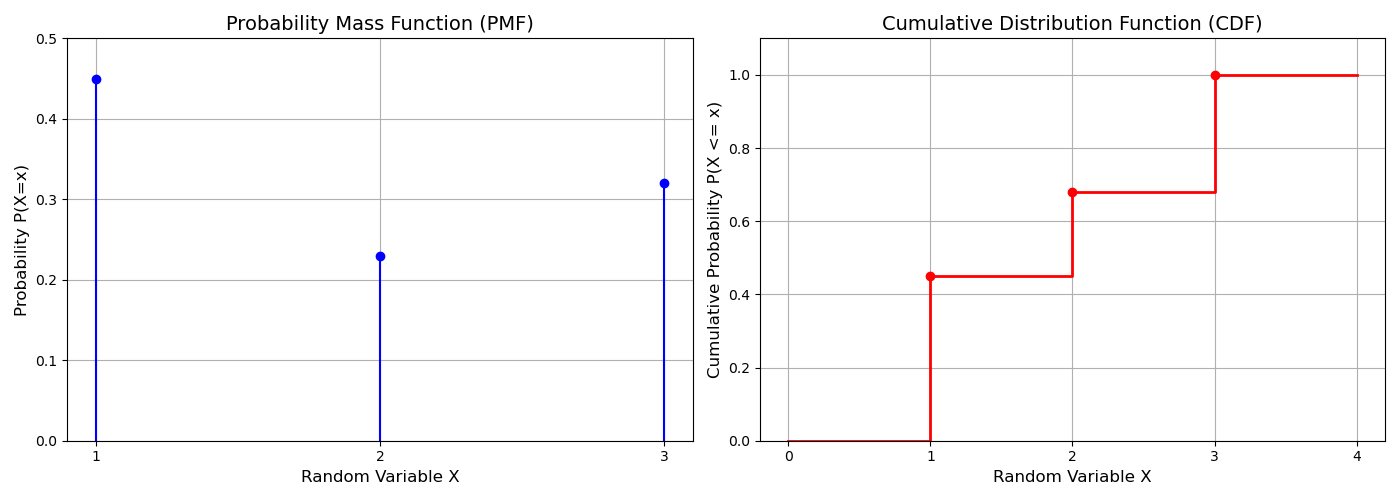
\includegraphics[width=\columnwidth, height=0.8\textheight, keepaspectratio]{figs/fig.png}   
\end{frame}



\begin{frame}[fragile]
    \frametitle{Python Code }
\begin{lstlisting}
import numpy as np
import matplotlib.pyplot as plt
from scipy.stats import norm

X = [1, 2, 3]
prob = [0.45, 0.23, 0.32]

samples = 100000
data = np.random.choice(X, size=samples, p=prob)
mu = np.mean(data)
sigma = np.std(data)

print(f"Theoretical Mean: 1.870  | Simulated Mean: {mu:.3f}")
print(f"Theoretical Std:  0.868  | Simulated Std:  {sigma:.3f}")

plt.figure()
bins = [0.5, 1.5, 2.5, 3.5]
plt.hist(data, bins=bins, density=True, alpha=0.5, color='blue', 
         edgecolor='black', label='Simulated Data Histogram')
\end{lstlisting}
\end{frame}

\begin{frame}[fragile]
    \frametitle{Python Code }
\begin{lstlisting}
x_axis = np.linspace(0, 4, 100)
gaussianCurve = norm.pdf(x_axis, mu, sigma)

plt.plot(x_axis, gaussianCurve, 'r-', linewidth=2, 
         label=f'Gaussian Overlay\n($\mu$={mu:.2f}, $\sigma$={sigma:.2f})')

plt.axvline(1.87,color = "yellow",linewidth=1)
plt.axvline(mu,color = "green",linewidth=1)

plt.title('Simulation of Discrete PMF vs Continuous Gaussian Overlay', fontsize=14)
plt.xlabel('Random Variable X', fontsize=12)
plt.ylabel('Probability Density', fontsize=12)
plt.xticks(X)
plt.legend()
plt.grid(axis='y', linestyle='--', alpha=0.7)
plt.show()
\end{lstlisting}
\end{frame}

\begin{frame}{Plot}
    \centering
    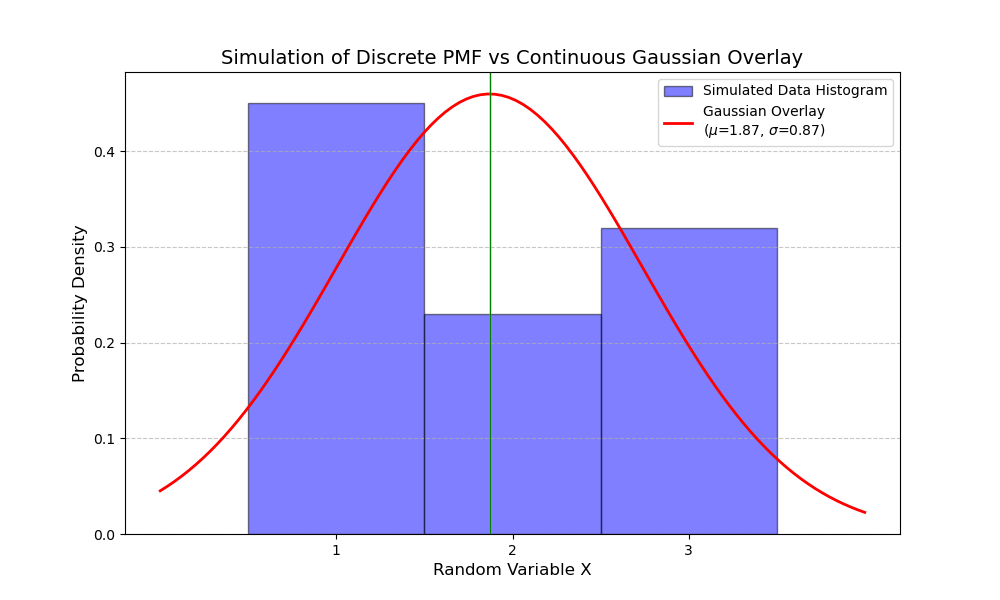
\includegraphics[width=\columnwidth, height=0.8\textheight, keepaspectratio]{figs/plt.png}   
\end{frame}


\end{document}
